\section{问题四的模型的建立和求解}
\subsection{问题四的描述与分析}

本问引入宏基站(Macro BS, 记作 MBS)与多个微基站(Small BS, 记作 SBS)的异构蜂窝网络:MBS 具备更充裕的频谱资源且覆盖广;SBS 负责边缘热点的增强覆盖。题设指出 MBS 与所有 SBS 采用不重叠频谱,因此跨层无干扰;但各 SBS 之间同频复用,存在相互干扰。
本问是一个“跨层接入 + 多站切片 + 切片级功率控制 + 队列与 SLA 约束 + SBS 间干扰耦合”的时变混合整数非凸优化问题(MINLP)。经过分析,上一问的模型框架在本问中得以延续,但需针对异构网络的特性进行调整。

\subsection{模型建立}
本问的模型延续之前的内容,但需要对信道与干扰模型、接入与调度规则、决策变量等进行调整,以适应宏基站与微基站的异构网络结构,相同的模型不再重复。

\subsubsection{信道与干扰模型}

本问的信道模型核心要素与前文一致,用户的瞬时接收功率 $p_{\mathrm{rx},n\to k}(\tau)$ 与热噪声功率 $N_0(i_s)$ 的计算公式保持不变。我们在此基础上,重点阐述第四问独特的异构网络干扰模型。

根据题目设定,宏基站(MBS, $n=0$)与所有微基站(SBS, $n \in \mathcal{N}$)工作在不同频段,因此它们之间不存在跨层干扰。干扰仅存在于同频部署的各个 SBS 之间。用户的信干噪比(SINR)$\gamma_k(\tau)$ 因此取决于其所接入的基站类型:
\begin{itemize}
    \item \textbf{当用户接入 MBS ($n=0$) 时},不存在干扰,其接收质量由信噪比(SNR)决定:
    \begin{equation}
        \gamma_k(\tau) = \frac{p_{\mathrm{rx},0\to k}(\tau)}{N_0(i_s)}, \quad \text{若 } a_{0,k}(t)=1
    \end{equation}

    \item \textbf{当用户接入 SBS ($n \in \mathcal{N}$) 时},会受到来自其他 SBS 的同频干扰。干扰功率 $I_{u\to k}(\tau)$ 来自于其他 SBS $u$ ($u \in \mathcal{N}, u \neq n$) 在相同 RB 上的发射。此时,信干噪比为:
    \begin{equation}
        \gamma_k(\tau) = \frac{p_{\mathrm{rx},n\to k}(\tau)}{\sum_{u \in \mathcal{N}, u \neq n} I_{u\to k}(\tau) + N_0(i_s)}, \quad \text{若 } a_{n,k}(t)=1, n \in \mathcal{N}
    \end{equation}
    其中,干扰项 $I_{u\to k}(\tau)$ 的计算方式与信号功率 $p_{\mathrm{rx}}$ 类似。
\end{itemize}

综合以上两种情况,用户 $k$ 在时刻 $\tau$ 的瞬时数据传输速率(bps)可由香农公式计算得出:
\begin{equation}
 r_k(\tau)=i_s\cdot b\cdot \log_2\big(1+\gamma_k(\tau)\big)
\end{equation}


\subsubsection{接入与调度规则}

本问的接入与调度在继承前问规则的基础上,引入了针对异构网络的特定限制:
\begin{itemize}
  \item \textbf{接入限制}:这是本问的核心特征。每个用户 $k$ 的接入选择被严格限定在宏基站(MBS)与地理位置最近的微基站(SBS)之间,即 $a_{n,k}(t)=1$ 仅在 $n=0$ 或 $n=n^*(k)$ 时才可能成立。
  \item \textbf{并发与调度}:各基站(MBS与SBS)的切片并发容量 $C_{n,s}(t)$ 的计算方式,以及窗口内“编号优先、任务完成即补位、URLLC按紧迫度优先”的调度机制,与前文保持一致。
\end{itemize}

\subsubsection{决策变量与优化模型}

决策变量:
\begin{itemize}
  \item RB 切片分配:$x_{n,s}(t)\in\mathbb{Z}_{\ge 0}$
  \item 发射功率:$p_{0,s}(t)\in[10,40]$ (dBm),$p_{n,s}(t)\in[10,30]$ (dBm)
  \item 接入关联:$a_{n,k}(t)\in\{0,1\}$,当 $a_{n,k}(t)=1$ ,则 $k$ 在窗口 $t$ 仅由站 $n$ 调度;若 $n\notin\{0,n^*(k)\}$, $a_{n,k}(t)=0$
\end{itemize}
综合上述要素,第四问的动态联合优化模型可表述为(跨 10 个窗口聚合):
\begin{equation}
\begin{aligned}
\max\limits_{\{x,p,a\}}\quad & Q_{\text{total}}=\sum_{t\in\mathcal{T}}\Bigg[\sum_{k\in\mathcal{K}_U}\sum_{\tau\in\mathcal{A}_k(t)} y^{U}_{k,\tau}+\sum_{k\in\mathcal{K}_e}\sum_{\tau\in\mathcal{A}_k(t)} y^{e}_{k,\tau}+\sum_{k\in\mathcal{K}_m}\sum_{\tau\in\mathcal{A}_k(t)} y^{m}_{k,\tau}\Bigg] 
\end{aligned}
\end{equation}

\begin{equation}
\text{s.t.}\quad 
\left\{
\begin{aligned}
& \sum_{s\in\mathcal{S}} x_{n,s}(t)=R_n\\
& x_{n,U}(t)\bmod 10=0,\ x_{n,e}(t)\bmod 5=0,\ x_{n,m}(t)\bmod 2=0\\
& x_{n,s}(t)\in\mathbb{Z}_{\ge 0}\\
& 10\le p_{0,s}(t)\le 40,\ 10\le p_{n,s}(t)\le 30\ (\forall n\in\mathcal{N})\\
& Q_k(t+100)=\max\Big\{0,\ Q_k(t)+\sum_{\tau\in\mathcal{F}(t)} D_k(\tau)-S_k(t)\Big\}\\
& r_k(\tau),\ \gamma_k(\tau)\ \text{由}\ (x,p,a)\ \text{与}\ (\phi,h)\ \text{及调度生成}\\
& \sum_{n\in\bar{\mathcal{N}}} a_{n,k}(t)\le 1\\
& \forall n\in\bar{\mathcal{N}},s\in\mathcal{S},t\in\mathcal{T},\ \forall k,t
\end{aligned}
\right.
\end{equation}
其中 $\mathcal{A}_k(t)\subseteq\mathcal{F}(t)$ 为窗口 $t$ 内属于用户 $k$ 且在 SLA 内完成的任务到达时刻集合。\\
该模型体现了“跨层接入选择 + 多站切片 + 切片级功率 + SBS 间互扰 + 任务队列”的耦合,属于时变 MINLP。

\subsection{模型求解}

第四问的优化模型在第三问的基础上引入了宏基站(MBS)与微基站(SBS)的异构结构,并增加了用户接入选择的约束。模型的决策变量维度、干扰关系和资源边界均发生了显著变化,使其成为一个更复杂的混合整数非线性规划(MINLP)问题。直接求解该问题在计算上是不可行的。

我们延续并拓展了问题三中“\textbf{滚动时窗预测控制(MPC)} + \textbf{混合编码遗传算法(GA)}”的求解框架。该框架的总体思想和流程与问题三(见图~\ref{fig:flow_q3})保持一致,即通过 MPC 将长时域问题分解为一系列独立的百毫秒窗口优化问题,再利用 GA 对每个窗口内的“用户接入+资源切片+功率控制”联合优化问题进行高效搜索。本节将重点阐述为适配第四问场景而对 GA 内核所做的关键修改,与问题三重复之处不再赘述。

\subsubsection{内层:混合编码遗传算法 (GA) 的适配}

针对每个决策窗口内的静态资源分配问题,我们对遗传算法的编码、适应度评估和算子进行了如下调整:

\begin{itemize}
    \item \textbf{个体编码方案}:每个个体(染色体)代表一个完整的资源分配策略,其混合编码结构调整如下:
    \begin{enumerate}
        \item \textbf{用户接入决策}:根据模型约束,每个用户在每个窗口只能选择接入宏基站(MBS)或距离其最近的一个微基站(SBS)。因此,该部分编码为一个长度为 48 的\textbf{二进制向量},其中基因位 $i$ 的值为 0 代表用户 $i$ 接入 MBS,为 1 则代表其接入该窗口起始时刻的最近 SBS。这相比问题三的接入决策空间有了大幅简化。
        \item \textbf{RB 切片分配}:编码为一个长度为 $2 \times 4 = 8$ 的整数向量。由于存在 1 个 MBS 和 3 个 SBS,共 4 个基站,我们为每个基站的 URLLC 和 eMBB 切片分配 RB 数量。MBS 的总 RB 数为 100,每个 SBS 为 50。mMTC 切片的 RB 数仍由总数减去 U/E 切片后剩余的资源确定,并向下对齐到切片粒度。
        \item \textbf{切片功率控制}:编码为一个长度为 $4 \times 3 = 12$ 的浮点数向量,分别表示 4 个基站上 3 个切片的发射功率(dBm)。MBS 的功率范围为 $[10, 40]$ dBm,而 SBS 的功率范围为 $[10, 30]$ dBm。
    \end{enumerate}

    \item \textbf{适应度函数}:个体的适应度评估依然通过一个精细的、步长为 1 ms 的窗口仿真器来完成。该仿真器根据解码后的策略进行模拟,但其核心的速率计算模块进行了关键更新:
    \begin{itemize}
        \item \textbf{异构干扰模型}:仿真器精确地实现了第四问的干扰关系。MBS 与 SBS 工作在不同频段,因此 MBS 上的用户不受任何来自 SBS 的干扰。反之,所有 SBS 在同频段工作,因此一个 SBS 上的用户会受到其他所有\textbf{正在服务的、占用同类切片}的 SBS 的同道干扰。
        \item \textbf{动态接入点}:在每个窗口开始时,会根据所有用户当时的坐标预先计算出各自的“最近 SBS”。GA 在解码接入决策时,将基于这一预计算结果来确定用户的具体接入基站。
    \end{itemize}
    最终,仿真器输出的 QoS 总分作为该个体的适应度值。

    \item \textbf{遗传算子与参数}:我们沿用了问题三中的精英保留策略、锦标赛选择、混合交叉(单点交叉用于离散的接入决策,算术交叉用于连续的功率和 RB 变量)、多模式变异(随机扰动或高斯扰动)以及最优解保留。为应对更复杂的问题,参数调整为:种群大小为 50,最大进化代数为 500,交叉概率 0.8,变异概率 0.3。
\end{itemize}

\subsection{结果分析}
我们采用上一节提出的“滚动MPC+GA”方法对问题四进行了求解,得到了10个决策窗口内每个基站的资源块(RB)分配、切片功率以及用户接入策略。详细的数值结果记录在代码附录的 \texttt{q4\_user\_bs\_mapping.csv} 和 \texttt{q4\_window\_results.csv} 文件中。本节将对这些结果进行分析。

\subsubsection{总体性能与动态适应性}
在1000ms的仿真周期内,我们所提出的算法实现了 \textbf{834.02} 的总服务质量(QoS)得分。每个窗口的详细QoS得分、资源和功率分配决策汇总于表~\ref{tab:q4_results}。

\begin{table}[H]
  \centering
  \caption{问题四各窗口资源分配决策与QoS结果(部分)}
  \label{tab:q4_results}
  \resizebox{\textwidth}{!}{%
  \begin{tabular}{c|ccc|ccc|ccc|ccc|c}
    \toprule
    \textbf{Win} & \multicolumn{3}{c|}{\textbf{MBS\_1 (RB/P(dBm))}} & \multicolumn{3}{c|}{\textbf{SBS\_1 (RB/P(dBm))}} & \multicolumn{3}{c|}{\textbf{SBS\_2 (RB/P(dBm))}} & \multicolumn{3}{c|}{\textbf{QoS}} & \textbf{Obj.} \\
    \cmidrule(lr){2-4} \cmidrule(lr){5-7} \cmidrule(lr){8-10} \cmidrule(lr){11-13}
     & \textbf{U} & \textbf{E} & \textbf{M} & \textbf{U} & \textbf{E} & \textbf{M} & \textbf{U} & \textbf{E} & \textbf{M} & \textbf{U} & \textbf{E} & \textbf{M} & \\
    \midrule
    0 & 30/25.1 & 40/23.8 & 30/24.6 & 20/24.6 & 20/25.8 & 10/25.0 & 20/25.0 & 0/27.8 & 30/26.2 & 93.42 & 14.26 & 40.00 & 147.68 \\
    1 & 30/25.7 & 0/25.2 & 70/26.9 & 0/25.5 & 0/27.5 & 50/24.1 & 30/25.9 & 0/22.3 & 20/24.0 & 85.68 & 0.00 & 40.00 & 125.68 \\
    2 & 50/25.8 & 0/24.1 & 50/22.9 & 0/28.1 & 0/26.0 & 50/23.3 & 0/19.9 & 0/26.8 & 50/25.1 & 64.61 & 0.00 & 40.00 & 104.61 \\
    3 & 0/22.5 & 0/22.7 & 100/23.3 & 30/21.0 & 0/24.7 & 20/21.1 & 30/26.4 & 0/21.9 & 20/25.7 & 50.85 & 0.00 & 40.00 & 90.85 \\
    4 & 0/24.9 & 0/24.8 & 100/27.8 & 0/25.5 & 0/29.2 & 50/21.0 & 30/23.7 & 0/25.9 & 20/24.1 & 43.16 & 0.00 & 40.00 & 83.16 \\
    5 & 0/21.2 & 0/26.5 & 100/25.9 & 30/30.0 & 0/25.9 & 20/23.1 & 30/25.6 & 0/24.7 & 20/27.0 & 50.27 & 0.00 & 40.00 & 90.27 \\
    6 & 0/22.0 & 0/29.6 & 100/22.4 & 20/25.8 & 0/24.9 & 30/24.1 & 30/27.6 & 0/22.2 & 20/25.5 & 47.51 & 0.00 & 40.00 & 87.51 \\
    7 & 0/27.4 & 0/24.9 & 100/29.0 & 20/26.3 & 0/28.5 & 30/20.9 & 30/25.1 & 0/29.4 & 20/26.5 & 48.32 & 0.00 & 34.10 & 82.42 \\
    8 & 0/23.2 & 0/22.8 & 100/26.9 & 10/24.2 & 0/21.9 & 40/29.4 & 20/23.8 & 0/26.8 & 30/23.9 & 19.48 & 0.00 & 10.03 & 29.50 \\
    9 & 0/22.3 & 0/23.9 & 100/29.8 & 30/22.3 & 0/25.6 & 20/26.0 & 50/23.9 & 0/28.4 & 0/29.3 & 11.74 & 0.00 & -19.38 & -7.64 \\
    \bottomrule
  \end{tabular}%
  }
\end{table}

从表~\ref{tab:q4_results}可以看出,算法在不同时间窗口展现出高度的动态适应性。
\subsubsection{宏基站与微基站的协同策略}
根据题目要求用户只能接入MBS或距离其最近的SBS,通过求解,我们得到了用户接入基站决策,如图\ref{fig:q4_user_bs_mapping}所示。
\begin{figure}[H]
    \centering
    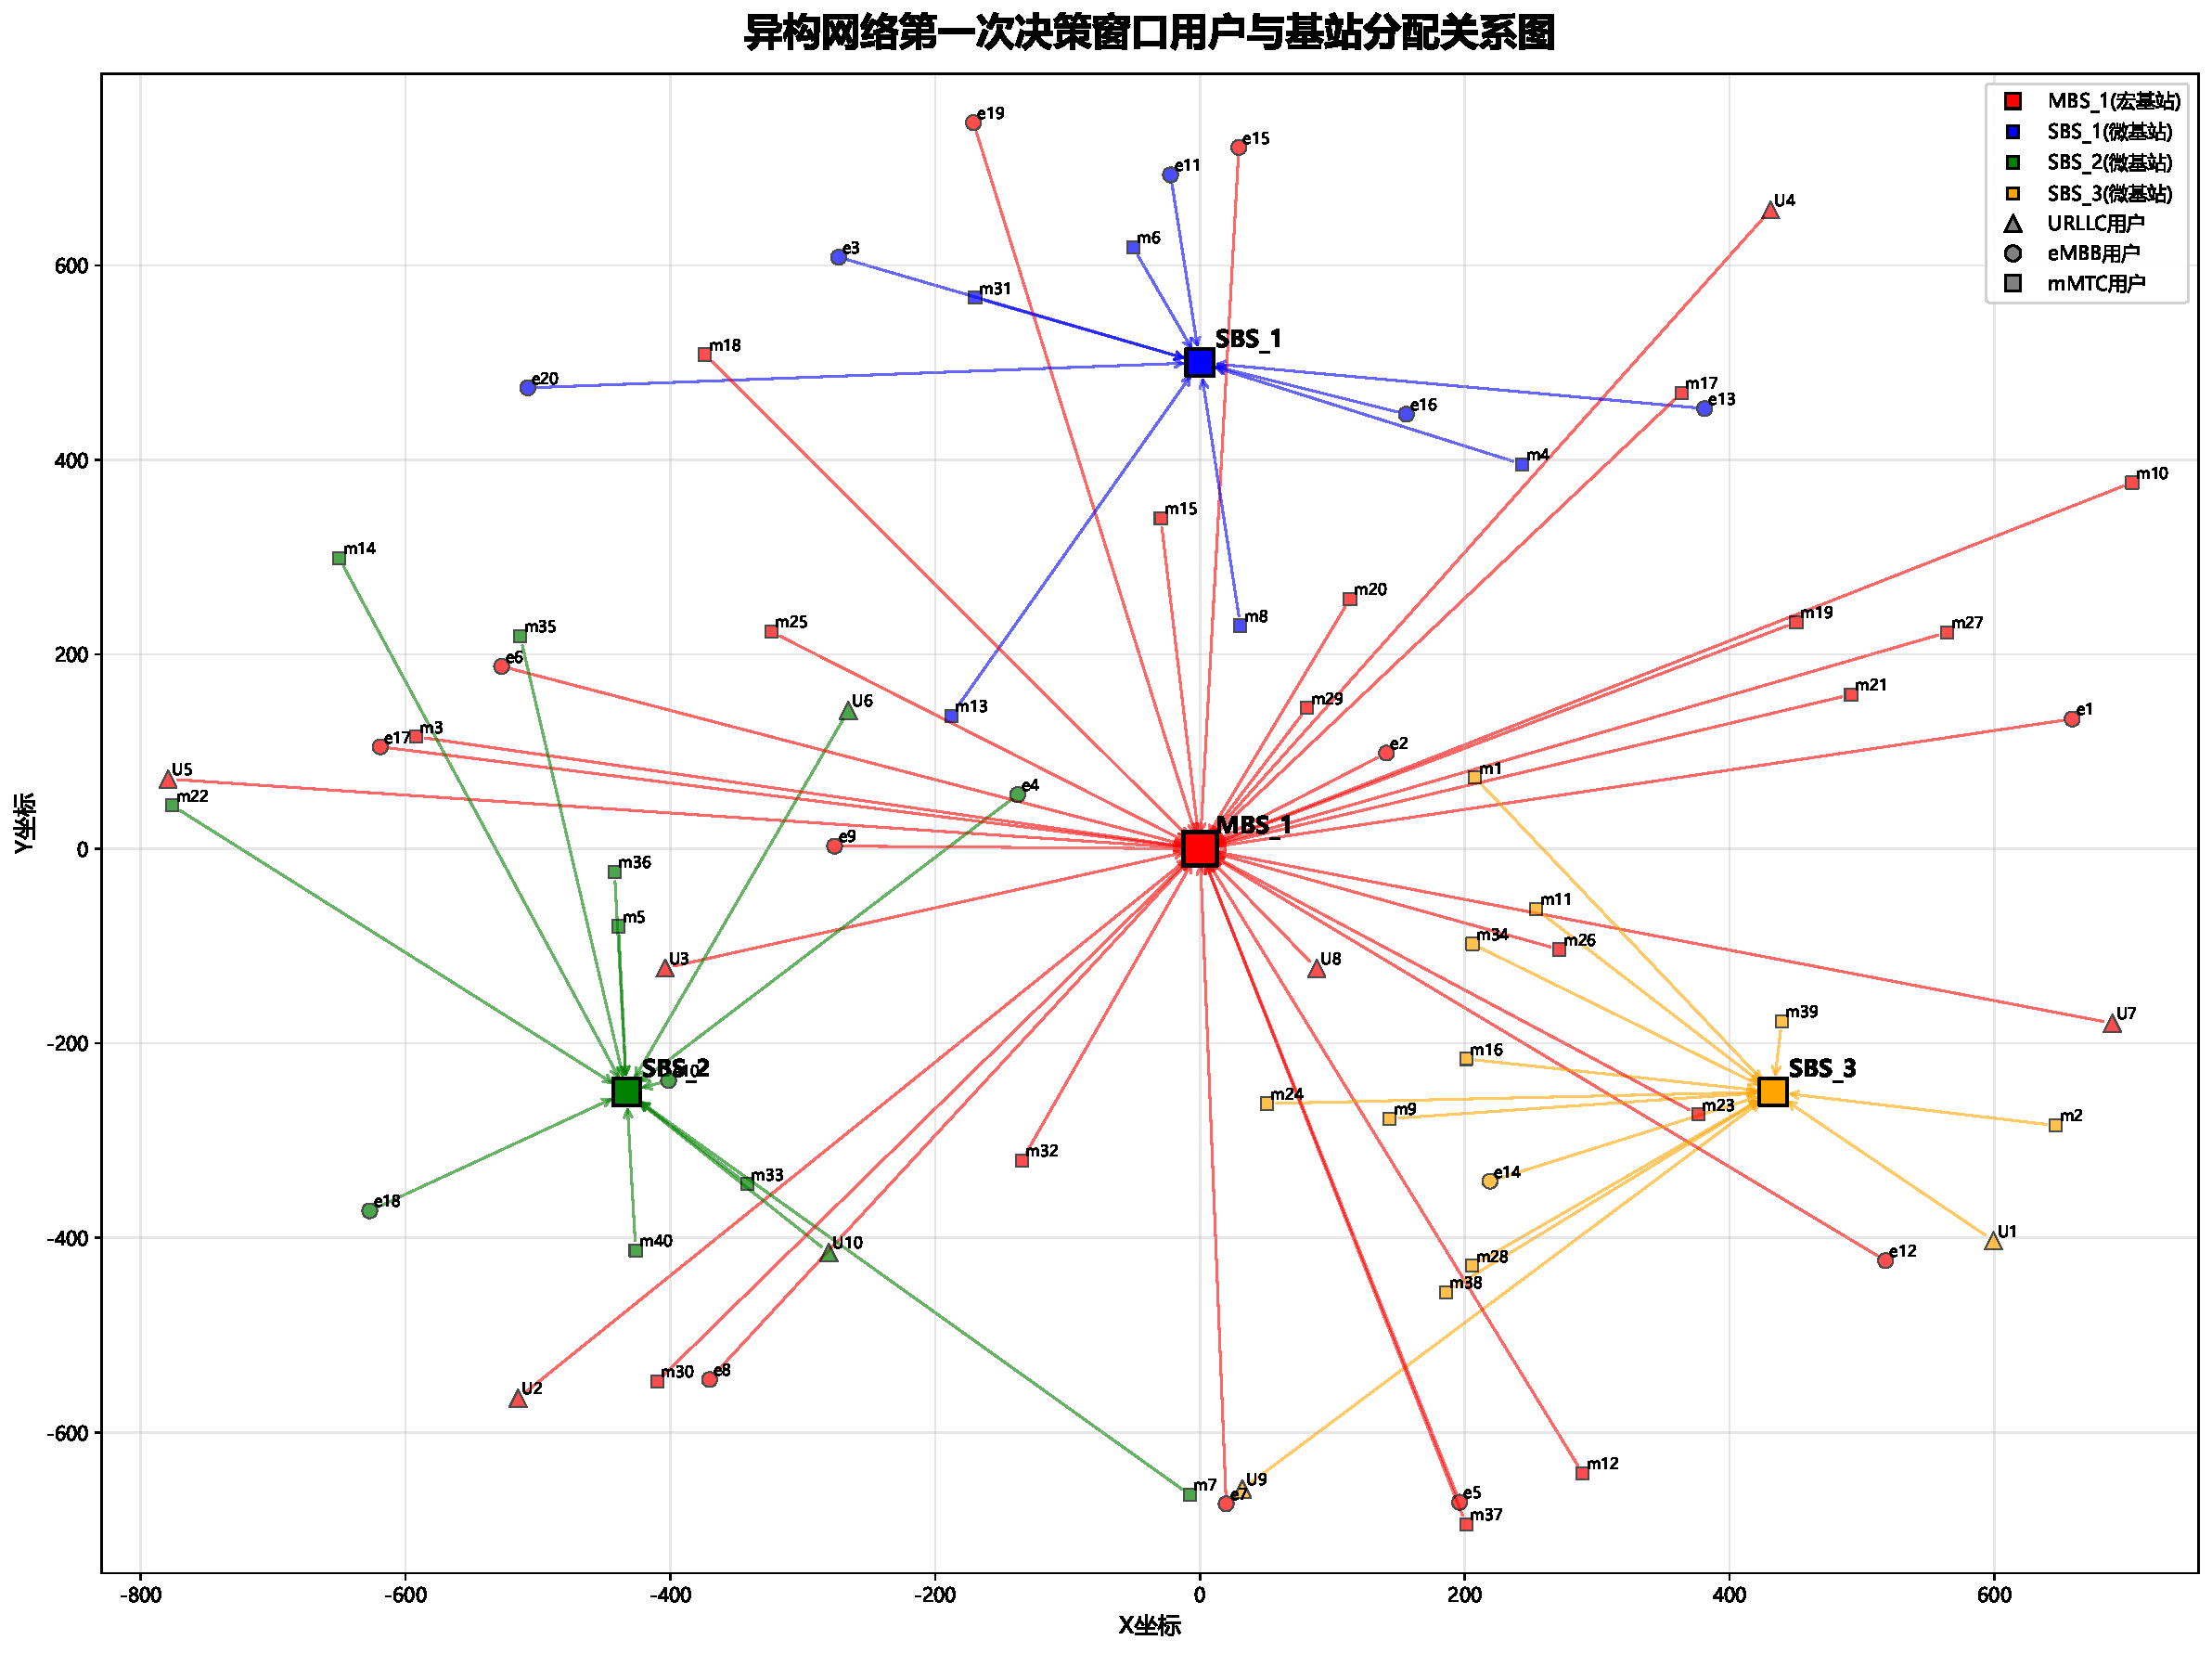
\includegraphics[width=0.85\textwidth]{figures/第四问结果可视化.pdf}
    \caption{第四问用户接入可视化}
    \label{fig:q4_user_bs_mapping}
\end{figure}

\begin{itemize}
    \item \textbf{宏基站(MBS)的角色}:MBS拥有100个RB和更高的功率上限(40dBm),且无干扰,是网络中的“定海神针”。算法倾向于利用MBS来处理大规模、可容忍一定时延的业务。从窗口1到9,MBS几乎将全部资源投入到mMTC切片,确保了mMTC业务在大多数窗口都能拿到满分(40分),这体现了利用MBS广覆盖、大容量优势来满足海量连接的策略。
    \item \textbf{微基站(SBS)的角色}:SBS资源有限(50个RB)且存在同频干扰,但其部署更靠近用户,能提供更好的信道条件。算法主要利用SBS来保障对时延和速率要求苛刻的业务。例如,在窗口3,当MBS全力服务mMTC时,三个SBS协同为URLLC用户提供了总计80个RB的资源,有效保障了高优先级业务的QoS。此外,SBS的功率控制也十分灵活,例如在窗口5,SBS\_1为URLLC切片输出了30dBm的满功率,以对抗干扰、确保可靠性。
\end{itemize}
